%% LyX 2.1.2.2 created this file.  For more info, see http://www.lyx.org/.
%% Do not edit unless you really know what you are doing.
\documentclass[english]{llncs}
\usepackage[T1]{fontenc}
\usepackage[latin9]{inputenc}
\usepackage{amsmath}
\usepackage{graphicx}

\makeatletter
%%%%%%%%%%%%%%%%%%%%%%%%%%%%%% Textclass specific LaTeX commands.
\numberwithin{equation}{section}
\numberwithin{figure}{section}

%%%%%%%%%%%%%%%%%%%%%%%%%%%%%% User specified LaTeX commands.
\usepackage {url}
\usepackage [numbers]{natbib}

\makeatother

\usepackage{babel}
\begin{document}

\title{Image Segmentation by Size-Dependent Single Linkage Clustering of
a Watershed Basin Graph }


\author{Aleksandar Zlateski\textsuperscript{1} and H. Sebastian Seung\textsuperscript{2}}


\institute{\textsuperscript{1} CSAIL, Massachussets Institute of Technology,
USA\\
\texttt{zlateski@mit.edu}\\
\textsuperscript{2} PNI, Princeton University, USA\\
\texttt{sseung@princeton.edu}}
\maketitle
\begin{abstract}
We present a method for hierarchical image segmentation that defines
a disaffinity graph on the image, over-segments it into watershed
basins, defines a new graph on the basins, and then merges basins
with a modified, size-dependent version of single linkage clustering.
The method is illustrated on the challenging problem of segmenting
3D electron microscopic brain images.

Our watershed transform works by finding the basins of attraction
of steepest descent dynamics, and has runtime that is linear in the
number of graph edges. It yields basins similar to those of watershed
cuts (Cousty et al. 2009), except that plateaus are divided between
basins consistently and in a more even way. In general, watershed
algorithms tend to produce severe over-segmentation, which can be
counteracted by pre- and/or post-processing.

Our post-processing starts by examining the new graph on the basins,
in which the edge connecting two basins is assigned the same weight
as the minimal edge connecting the basins in the original disaffinity
graph. Then single linkage clustering yields a hierarchical segmentation
of the original image in which the lowest level consists of the watershed
basins. The levels of single linkage clustering yield flat segmentations
in which some of the basins are merged.

If we only expect to use levels above some minimum value T\_min, then
it turns out to be equivalent and more efficient to preprocess the
original disaffinity graph before watershed by setting all edge weights
below T\_min to a common low value. In another pre-processing step
we remove the edges with disaffinity to allow for unsegmented regions.

We also show how to modify single linkage clustering by making it
depend not only on edge weights but also on cluster size - volume,
length, etc. The modification is useful when there is prior knowledge
about the size of true segments, and is shown to have an efficient
implementation because size is a property that is guaranteed to increase
with each agglomerative step.

\medskip{}


\textbf{Keywords: }Watershed, image segmentation, graph, electron
microscopy
\end{abstract}


\section{Introduction}

\cite{Cousty2009,Cousty2010,Cousty2011,Falcao2004,Felzenszwalb2004,Guimaraes2012,Mustafa,Punnen1991,Wassenberg2009}\cite{Cousty2009,Cousty2010,Cousty2011,Falcao2004,Felzenszwalb2004,Guimaraes2012,Mustafa,Punnen1991,Wassenberg2009}

The watershed algorithm is widely used for segmenting images (cite),
and has also been generalized to the partitioning of graphs (cite).
In this paper we will focus on watershed for affinity graphs, which
is relevant for the special case of images. However our results are
applicable to arbitrary graphs. 

The standard watershed algorithm produces as many segments as there
are local minima. In a case of noisy data (e.g. images) there will
be a lot of local minima leading to lots of small segments {[}image{]}.
A proposed solution to deal with the noisy data is to, instead of
applying regular watershed, first connected components are applied
to the thresholded graph, after which marker watershed is performed.
The number of components will be equal to the number of components
of the thresholded graph. The problem with this approach is that it
doesn\textquoteright t generate a hierarchical segmentation - it pre-determines
the number of segments. Moreover, the same result can be generated
from the hierarchy obtained with our algorithm by merging segments
until we reach the same number of segments.

The standard watershed algorithm produces a set of segments (set of
nodes) from which we can easily obtain a region graph and a hierarchical
segmentation (MST of the region graph). The edges of the graph connecting
the segment are the min-max edges between the pairs of the nodes in
the two component.

\textbf{Degeneracy Issue}

We solve the degeneracy problem by assigning a graph node to be part
of the same segment as the closest node at the edge of the non-minima
plateau. In the 2D or 3D affinity graph case that would be equal to
the closest border node by manhattan distance. In a case of tie we
pick a random segment. The details of the algorithm are explained
in the Algorithm section.

\textbf{Extending the Watershed Algorithm}

We extend the watershed algorithm by adding a set of rules about merging
the original watershed segments. Some of the rules can be applied
during the initial phase, while the original watershed segmentation
is computed and thus it doesn\textquoteright t have any additional
computational cost. Other can be applied on the applied by a single
linear pass through the region graph.

\textbf{Introducing Thresholds.}

The first set of extensions we introduce is a set of thresholds. Specifically
we will introduce the following thresholds. High threshold, the edges
with the value greater or equal to the high threshold value will be
collapsed. Low threshold - the edges with the value lower than the
low threshold will never be collapsed. Size threshold - if any of
the two segments that are connected in the resulting region graph
are smaller than the size threshold will be merged. The order of the
merging will be decided by the value of the edges - higher values
will be merged first.

\textbf{Arbitrary Properties and Merging Function}

We further extend the watershed algorithm by introducing merging functions
and properties. The function F(a,b), where a and b are the properties
of two connected segments in the region graph represents the lowest
possible value of the edge for which the two component should be merged.
The function F(a,b) has to be strictly non decreasing in order to
avoid ambiguous results. a and b are properties of the two segments
(e.g. sizes in number of nodes, center of mass, etc..). In order to
keep the efficiency of the algorithm we require that computing the
property of the segments created by merging two segments must be done
in constant time. In the case of the size it is a simple sum of two
numbers.

\textbf{Recursive Application (Extending it even further)}

Another approach to deal with the excessive noise is to recursively
apply the watershed algorithm on the obtained region graph. As described
our watershed algorithm can be applied to an arbitrary graph, and
therefore it can be applied on the results of a watershed. The approach
is especially useful for very noisy data for which we don\textquoteright t
have any prior knowledge. This approach can be combined with the previously
described extensions.


\section{Watershed transform definition}

Roughly speaking we want to define the steepest descent stochastic
discrete dynamics on an undirected weighted graph and then partition
the graph into the basins of attraction of this dynamics. But there
are sproblems!

The vertices of the graph represent the states of our system. For
a given state $u$ in the next timestep the system evolves into a
state $u$if there is an edge $\{u,v\}$ in our graph such that the
weight of the edge is not larger than any edge containing $u$. If
there's multiple states satisfying the condition, the system can evolve
into any of them with equal probability.

We will have one basin of attraction for each regional minima.

Problem - stationary points in the dynamics which correspond to non-minima
plateaus.

There might be more than one steepest descent path from a vertex going
to distinct regional minima. A vertex can have two basins of attraction.

We will solve this problem by introducing border vertices.

Let's describe our stochastic dynamic on the given weighted graph
G.



For a given initial state $v_{0}$ the evolution of the system can
be represented as an infinite \emph{steepest descent walk} $v_{0},e_{0},v_{1},e_{1},v_{2},\dots$

A \emph{steepest descent path} is a \emph{steepest descent walk }with
no repeating vertices except possibly the first and the last vertex.

For every \emph{steepest descent walk} there exist a \emph{steepest
descent path} containing the only the subset of the vertices and the
edges of the \emph{steepest descent walk.}

An edge between vertices $u$ and $v$ \emph{is locally minimal }if
its weight is not larger than the weights of all edges containing
either $u$ or $v$.

A \emph{regional minimum }of a graph is a connected component of the
subgraph containing only the locally minimal edges\emph{ }such that
every possible steepest descent walk in $G$ starting in any of the
vertices of the connected component\emph{ }stays inside the component.

If the graph doesn't have any isolated vertices then every initial
state of the system will, after a finite number of steps, be trapped
into a regional minimum.
\begin{proof}
First 

A \emph{basin of attraction} of a \emph{regional minimum} is a set
of vertices from which there is a \emph{steepest descent path} to
every vertex of the \emph{regional minimum}.


\emph{Basins of attraction }of different \emph{regional minima} can
overlap. A vertex can belong to more than one \emph{basin of attraction}.


A \emph{border vertex} is part of more than one \emph{basin of attraction.}


Let $B$ be a set of all \emph{border vertices}. For every \emph{basin
of attraction }$A_{i}$, the set $A_{i}\backslash B$ is defined as
the \emph{basin of strong (exclusive) attraction} of the same \emph{regional
minimum}.


The\emph{ }watershed\emph{ }transform of a graph is a collection of
watershed domains, where a domain is a basin of strong (exclusive)
attraction of a regional minimum. The border vertices are called the
ridges of the watershed transform.

\end{proof}

If the edge weights of a graph are distinct, then the watershed transform
will not have any ridges.

All but isolated vertices will be assigned to a \emph{domain}.


\section{Standard watershed algorithm}

The central quantity in the watershed algorithm is the steepest descent
graph, defined as follows.

Consider an undirected weighted graph $G$. Define the directed graph
$G'$ in which each undirected edge of $G$ is replaced by both directed
edges between the same vertices. The \emph{steepest descent graph}
$D$ is a subgraph of $G'$ with the property that $D$ includes every
edge of $G'$ with minimal weight of all edges outgoing from the same
vertex. 

A directed path in $D$ is a path of steepest descent in $G$, in
the sense that every step is along an edge with locally minimal weight.
The steepest ascent graph can be defined analogously using edges of
maximal weight. The watershed algorithm is named because a drop of
water is imagined to take a path of steepest descent on a landscape.
Either steepest ascent or descent can be used without loss of generality.

All the outgoing and bidirectional edges of a vertex of $D$ will
have smaller weight than all incoming vertices.

Every non-isolated vertex of $D$ will have at least one bidirectional
or outgoing edge.

The evolution of our stochastic descrete dynamics is equivalent to
a random walk along the\emph{ steepest descent graph}.

A \emph{saddle vertex} of the steepest descent graph has more than
one outgoing edge.

A \emph{plateau} is a connected component of the subgraph of $A$
containing only bidirectional edges.

The smallest possible plateau consists of two vertices, with a bidirectional
edge between them.

All the bidirectional edges inside a plateau will have the same weight.

A \emph{plateau corner} is a \emph{plateau }vertex with one or more
outgoing edges\emph{.}

All the outgoing edges off all \emph{plateau} corners of a single
plateau have the same weight equal to all the bidirectional edges
inside the plateau.

A \emph{locally minimal plateau }contains no \emph{plateau corners. }

A locally minimal plateau of the steepest descent graph is the same
as the regional minimum of the original graph.

A \emph{non-minimal plateau }contains at least one \emph{plateau corner}.

A \emph{compressed steepest descent multigraph }(CSDM) is obtained
by collapsing \emph{plateaus} into \emph{super-vertices.} All the
bidirectional edges inside the plateau are removed and all the incoming
and outgoing edges are preserved.

We will refer to the \emph{super-vertices }obtained by collapsing
\emph{plateaus} as \emph{locally minimal }and \emph{non-minimal} \emph{super-vertex}
accordingly.

All the outgoing edges of a \emph{super-vertex} will have the same
weight, equal to all the bidirectional edges inside the plateau and
smaller than the weight of all incoming vertices.

The \emph{compressed steepest descent multigraph }will contain no
bidirectional edges. All but \emph{locally minimal super-vertices}
will have at least one outgoing edge.

Every directed path in the CSDM will have strictly decreasing weights
and will terminate in one of the \emph{locally minimal super-vertices}.


\subsection{The standard watershed algorithm }
\begin{enumerate}
\item We create the \emph{compressed steepest descent multigraph}.
\item We reverse the directions of all the edges.
\item We visit the vertices (and super-vertices) in a topological order.
When visiting a vertex we:

\begin{itemize}
\item If the vertex has no outgoing edges we assign a new unique domain
ID to it.
\item Otherwise, if all the vertices pointed to by the outgoing edges have
the same ID we assign the current vertex that ID, otherwise we assign
a special ID representing a border.
\end{itemize}
\item We assign all the vertices of the original graph. The plateau vertices
will be assigned to the same ID as the corresponding \emph{super-vertex}.
\item {*}If there is a single unique domain assign all the vertices of the
graph to that ID.\end{enumerate}
\begin{theorem}
\emph{The algorithm 3.1 will:}\end{theorem}

\begin{enumerate}
\item Assign each vertex in $G$ a unique domain corresponding to the regional
mimimim to which the system will evolve. If the system can evolve
to multiple regional minima, the vertex will be marked as a ridge
vertex.
\item The total number of domains will be equal to the number of \emph{locally
minimal plateaus} (\emph{regional minima)}.
\item All vertices in a \emph{locally minimal plateau }will be assigned
to the same \emph{domain}. Vertices in different \emph{locally minimal
plateaus }will be assigned to different \emph{domains}.
\item All \emph{Domains }will be connected.\end{enumerate}
\begin{proof}
The step 3 of the algorithm assigns a unique domain ID only to vertices
with no outgoing edges. Only \emph{locally minimal super-vertices}
have no outgoing edges and therefore will be assigned a new unique
ID. As they correspond to\emph{ locally minimal plateaus }every \emph{locally
minimal plateau} will be assigned a different ID and all the vertices
in the \emph{plateau} will be assigned to that same ID. As we visit
the vertices in a topological order when visiting vertices that have
outgoing edges all the vertices pointed to by those edges will already
be visited and assigned. If they are all assigned to the same ID not
equal to the special ID representing a border then we know that all
the paths from the current vertex will terminate 
\end{proof}

Every path of the steepest descent graph is a non-increasing and terminates

\emph{Each vertex in }$G$ \emph{will be assigned to a unique domain
corresponding to the closest regional minimum by minimax distance
or will be designated as a border vertex. The total number of domains
will be equal to the number of }locally minimal plateaus\emph{. }All
vertices in a \emph{locally minimal plateau} \emph{will be assigned
to the same }domain. \emph{Vertices in different l}ocally minimal
plateaus\emph{ will be assigned to different }domains\emph{. Domains
will be connected.}
\begin{proof}
Prove this.
\end{proof}

If the steepest descent graph contains no saddle vertices or non-minima
plateaus with more than one plateau corner the watershed transform
will yield no non-isolated border vertices.

The isolated vertices of the original graph have an infinite distance
to all the other vertices. If the graph contains only one \emph{locally
minimal plateau} we will have only one \emph{domain, }and all the
vertices including the isolated ones will be assigned to it. If the
graph contains more than one \emph{locally minimal plateau} the isolated
vertices will be assigned as borders.

All the vertices in a \emph{non-minimal plateau }containing exactly
one \emph{plateau corner} will be assigned to the same domain as that
corner, if the corner belongs to a domain, or as borders if the corner
vertex is a border vertex.



The vertices in a \emph{non-minimal plateau} with more than one \emph{plateau
corner }will be assigned the special ID representing a border.




\section{Assigning border vertices}

The number of border vertices can be arbitrarily large. We would like
to assign the non-isolated border vertices to the domains in some
consistent and intuitive way. 
\begin{enumerate}
\item Not have degeneracies - have a deterministic algorithm.
\item All domains should be connected.
\item Plateaus should be fairly divided.
\end{enumerate}

\subsubsection*{Algorithm for dividing borders}
\begin{enumerate}
\item We introduce an ordering function $I$ of a graph $G=(V,E,W)$. $I:V\to\{1,2,...,|V|\}$
such that $I(u)\neq I(v)$ iff $u\neq v$. We'll refer to $I(u)$
as the index of $u$. 
\item We then modify the steepest descent graph and the original graph in
the following way:

\begin{enumerate}
\item For saddle vertices we keep only one outgoing edge pointing to $u$
with the minimal index.
\item We cut the non-minima plateaus with more than one plateau corner

\begin{enumerate}
\item For all non corner vertices that are we will keep a single bidirectional
edge (explain a bit clearer)
\item We remove all edges that have the two vertices equidistant to two
different plateau corners.
\end{enumerate}
\end{enumerate}
\end{enumerate}
\emph{The }standard watershed transform \emph{of the modified graph
will}
\begin{enumerate}
\item Uniquely assign all non-isolated vertices to a domain.
\item A vertex inside a \emph{non-minimal plateau} will be assigned to the
same \emph{domain} as one of the nearest \emph{plateau corners}.
\item The \emph{minimax distance} from any vertex to its assigned \emph{regional
minimum} will not be changed by the graph modification. (There exists
at least one minimax path of he original graph will remain in the
modified graph). Remark: Minimax distances can not decrease (b/c we
are only eliminating edges)

\begin{enumerate}
\item Remark: This is what the clames above mean: Every non-isolated border
vertex of the original graph was equidistant from multiple regional
minima. In the modified graph it has a unique closest regional minima
with unchanged minimax distance. The distance to the other regional
minima had increased.
\end{enumerate}
\end{enumerate}
\begin{proof}
Sketch: 1) Show that there's always non-decreasing path from a local
minima to a vertex. If there's a minimax path to two different local
minima then we didn't actually split the plateaus. 2) by design 3)
by design of the algorithm, we visit the graph using BFS 4) the value
of the removed edges will still be there.
\end{proof}


\section{Improving the watershed segmentation}

The edges of the graph usually represent \emph{affinities }or \emph{dissafinities
}- probabilities that the two vertices belong or don't belong to the
same segment. The watershed transform will produce a domain for every
regional minima. And slight noise in the data can therefore produce
large number of domains. Our goal is to reduce the number of segments
while still not getting mergers to improve the resulting segmentation.
In order to do this we will modify the \emph{dissafinity }graph for
the confident values.


\subsection{Minimum threshold $T_{\min}$}

For very small values of \emph{dissafinity} for which we are confident
that the two vertices should belong to the same domain we will modify
the \emph{dissafinity }value to be as low as possible. Mainly we will
modify the graph by replacing all edges with weight smaller than $T_{\min}$with
an edge with weight $0$. This will reduce the number the number of
domains as it will flatten the regions with small \emph{dissafinities},
reducing the noise.
\begin{enumerate}
\item Some regional minima will get merged into a larger one.
\item Other regional minima with the value larger or equal to $T_{\min}$
will stay.
\end{enumerate}
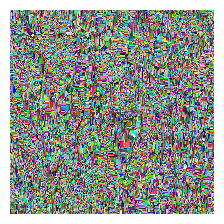
\includegraphics{Figures/raw} 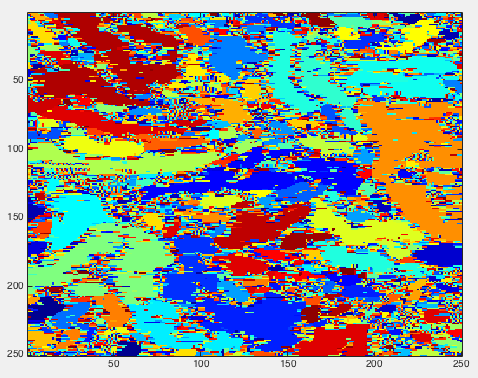
\includegraphics{Figures/min}


\subsection{Maximum threshold $T_{\max}$}

Similarly for very high values of dissafinity we can be confident
that the two vertices don't belong to the same domain. We can therefore
safely remove these edges from the graph. Removing edges with value
larger than $T_{\max}$can prevent some mergers. Also in the case
where the segments can have boundaries - vertices that shouldn't belong
to any of the segments the maximum threshold will produce small or
singleton segments where the boundaries should be.

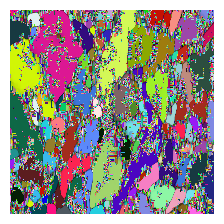
\includegraphics{Figures/minmax}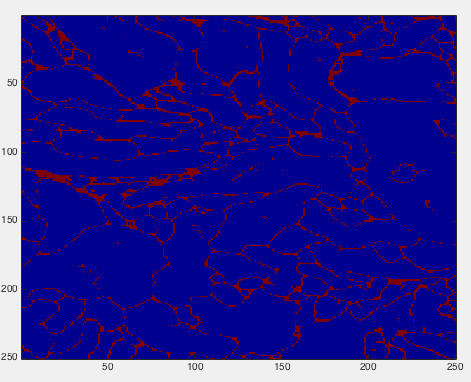
\includegraphics{Figures/singletons}


\subsection{Chosing $T_{\min}$and $T_{\max}$ values}

Not exact science :) get the largest possible values while not introducing
mergers. Further modification can make this choice be looser.


\section{Domain graph and hierarchical clustering}

A \emph{domain graph} $R=(D,E_{r},W_{r})$ of a partitioned graph
$G$ is an undirected weighted graph defined as follows 
\begin{enumerate}
\item The set of vertices $D$ is the set of domains/partitions of $G$.
\item $E_{r}\subset D\times D$.
\item The edge $\{d_{a},d_{b}\}\in D\times D$ exists iff $d_{a}\neq d_{b}$
and there exist an edge $\{v_{x},v_{y}\}$ in $G$ such that $v_{x}$
and $v_{y}$ are assigned to domains $d_{a}$ and $d_{b}$ accordingly.
\item The weight of the edge $\{d_{a},d_{b}\}$ is a real number determined
by $W_{r}(G,d_{a},d_{b})$ where $G$ is the original graph and $d_{a},$$d_{b}\subset V$
are the sets of vertices of the two domains.
\end{enumerate}
A \emph{standard? domain graph} is a \emph{domain graph }with $W_{r}(G,d_{a},d_{b})\equiv W_{\min}(G,d_{a},d_{b})\equiv\min\{W(\{u,v\}),u\in d_{a},v\in d_{b},\{u,v\}\in E\}$. 

A \emph{(standard) watershed domain graph} is a \emph{(standard) }domain
graph of a graph partitioned by the \emph{watershed transform}.

The edges of the \emph{standard watershed domain graph} will have
the weight equal to the minimax distance in $G$ between the \emph{regional
minima} of the corresponding domains.

The weights of the edges of the \emph{standard} \emph{domain graph}
of partitioned $G$ will have the value equal to the \emph{dissaffinity}
of the two closest members.


\subsection{Single linkage hierarchical clustering}

Given a graph $G$, hierarchical clustering treats each vertex as
a singleton cluster, and successively merges clusters until all partitions
have been merged into a single remaining cluster. A hierarchical clustering
is often represented as a dendrogram {[}fig{]}. Each merge operations
produces a new graph partition at the given level of the hierarchy.

In \emph{single linkage} hierarchical clustering in each step we merge
two clusters whose two closest members have the smallest \emph{disaffinity}.

In each step of the \emph{single linkage clustering }the values of
the \emph{smallest disaffinity} for which we merge the clusers will
be non-decreasing.

The graph partitioning obtained by \emph{single linkage} clustering
by merging clusters until the next smallest \emph{disaffinity} is
greater or equal to some threshold $T$ will be equivalent to the
partitioning obtained by obtaining the connected components of the
thresholded graph, where we only keep edges with weight smaller than
$T$.


\subsection{Relation between \emph{single linkage clustering and the watershed
transform}}

Explicitly explain that this is for a level of the hierarchical clustering. 

Graph partitioning is obtained by CC. 

Often a segmentation is produced using \emph{single linkage} \emph{clustering}
- connected components of the thresholded graph. An obvious problem
there is that this method can produce a lot of clusters. Each vertex
with that has no edge with the weight smaller than $T$ will be in
its own segment. A method to reduce the number of small, singleton
clusters is to apply the watershed transform on the resulting \emph{domain
graph}.

For a given threshold $T$, the following three methods will produce
the same partitioning of $G$
\begin{enumerate}
\item First partition the graph by finding the connected components of the
thresolded $G$ and then applying watershed on the resulting domain
graph.
\item Applying the watershed transform on $G$, and then finding the connected
components of the thresholded watershed domain graph.
\item Replacing all the edges with weight smaller than $T$ with an edge
of weight $0$ and then applying the watershed transform.\end{enumerate}
\begin{proof}
Prove this!

Explain why we want Watershed and then CC. or sometimes 3)
\end{proof}


\section{Methods for agglomerative clustering}

Often a prior knowledge about the nature of the data can be used to
improve the segmentation. In this section we introduce several efficient
methods.


\subsection{}






\subsection{Segment properties (modification of single linkage clustering + explain
the relationship)}

In many cases some properties of the desired segments are known. For
example, when segmenting neural tissue we can estimate the minimal
size of the segments inside a given volume.

A non-decreasing property $P:2^{V}\to R^{+}$ is a function of a segment
such that $P(S)\le P(S\cup v)$. Similarly we can define non-increasing
properties.

Exmple of non-decresing properties are size (number of vertices) in
the segment, bounding box volume (in the case of volumetric affinity
graphs), etc...

Given a property $P$ and prior knowledge about the data - $P(S)\ge P_{\min}$.
We propose the following method to improve the segmentation.
\begin{enumerate}
\item We consider all the edges of the standard domain graph in non-decreasing
order.
\item If the edge is connecting two different segments $S_{1}$ and $S_{2}$
and if either $P(S_{1})<P_{\min}$or $P(S_{2})<P_{\min}$. We merge
the segments $S_{1}$and $S_{2}$.
\end{enumerate}
In the algorithm described above it is enough to consider just the
edges of the minimum cost spanning forest of the domain graph.
\begin{proof}
Simple...

The method above does not take into account the wights of the edges
of the domain graph. P\_min as function of the weight.
\end{proof}


\subsection{Watershed hierarchical segmentation}

A \emph{watershed domain forest} is a \emph{minimum cost spanning
forest }of $R$, which is a union of \emph{minimum cost spanning trees}
of its connected components.



Algorithm for computing the forest. Then explain that the forest implies
a hierarchical segmentation.



Applying standard techniques for weighted graph clustering on the
watershed domain graph we obtain the watershed hierarchical segmentation.
We can do this in the following way: we consider all the edges in
the watershed domain graph in decreasing order. If the edge is connecting
two different domains we merge the two domains into a new domain.
The resulting partitioning of the graph will be our new level of hierarchical
segmentation. This algorithm is equivalent to the Kruskal's algorithm
for obtaining the maximum cost spanning forest so we can get both
the hierarchical segmentation and the watershed domain forest at the
same cost.

In the special case when $W_{r}(C_{a,b})$ is equal to the minimal
value of all the edges in $C_{a,b}$we can obtain the watershed domain
forest and the watershed hierarchical transform without creating the
watershed domain graph by considering all the edges of the original
graph $G$ in decreasing order and applying the same technique as
above. Note this is computationally more expensive (log factor).



The edges of the watershed domain forest will be a subset of a minimum
spanning forest of the original graph. Not explained correctly, need
better statement here.




\section{Agglomerative hierarchical clustering}

Often the result of the \emph{watershed transform }will produce an
oversegmentation. We will apply single-linkage clustering methods
on the \emph{watershed domain graph}. The \emph{watershed domains}
will represent the clusters and the weights of the edges of the \emph{watershed
domain graph }will represent the distance between the clusters.

A\emph{ minimax} \emph{path} between two vertices of a graph is a
minimum with respect to paths between the two vertices of the maximal
weight of edges on the path.

The\emph{ minimax distance} $d(u,v)$ between two vertices $u$ and
$v$ is equal to the maximal edge weight on a \emph{minimax path}
between the vertices. If no path between the two vertices exists,
then $d(u,v)=\infty$. The \emph{minimax }distance of a vertex to
itself is defined to be $0$.

The \emph{watershed domains }are the basins of attraction of the \emph{regional
minima}. 

- In the special case when the edge weight is chosen to be the minimum
of .... 

edge weight domain graph corresponds to the minimax distance between
any two pairs of points of the regional minima (between regional minima)

- more efficient

{*}difference between MCST. MCST has more information than the dendrogram.
MCST -> dendrogram. Kruskal's more powerful.

{*} two domains are in the same cluster iff the minmax distance between
the regional minima 

1) Relate CC of the two graphs

2) Relate the MST of the two graphs

3) Watershed on the domain graph on CC is the same as CC on the watershed
domain graph

In the case of segmentation, very often the edges of the given graph
represent \emph{disaffinities} - the measure of the likelihood that
the two vertices have similar characteristics, belong to the same
segment. Without losing generality we will assume that the small values
mean high likelihood. A slight noise in the affinity values can lead
to large number of regional minima producing large number of watershed
domains. We introduce modifications to the standard watershed algorithm
to deal with such noise.


\subsection{Maximum threshold}
\begin{enumerate}
\item Without losing generality, affinities take values {[}0,1{]} representing
probabilities of two vertices not belonging to the same segment.
\item We expect segment boundaries - vertices separating segments, not assigned
to any segment.
\item We are confident that the disaffinities larger than some value $T_{\max}$
should never be used to assign vertices to the same domain.
\end{enumerate}

\subsection{Minimum threshold}
\begin{enumerate}
\item Noisy data produces large number of regional minima and therefore
large number of watershed domains.
\item The hierarchical segmentation is useful only for a subset of thresholds,
we'll never use the hierarchical segmentation with a threshold smaller
than some value
\item A level of the hierarchical segmentation is obtained by merging watershed
domains starting from the watershed domain graph.
\item We can always increase the threshold, but never decrease (we have
to recompute the domain graph starting from the original graph)
\item Solutions

\begin{enumerate}
\item Do watershed transform and then compute the minimal level of the hierarchical
segmentation
\item Introduce the threshold before the watershed transform by replacing
all the edges....
\end{enumerate}
\end{enumerate}

\subsection{Relation to connected components}

An often used method for segmentation is applying connected components
on a thresholded graph. The resulting segmentation might produce a
lot of isolated vertices. Applying the watershed transform after introducing
the minimum threshold will produce a similar segmentation where all
vertices will be assigned either by growing existing connected components
of the thresholded graph or by introducing new segments.

Each connected component of the thresholded graph will be a subset-equals
to a single domain obtained by watershed followed by thresholding
the domain graph to the same threshold.

Doing marker based watershed which is not defined would be equivalent
to doing marker based watershed on the domain graph after thresholding
it.

Two domains of the tresholded domain graph will be in the same connected
component iff the two regional minima are in the same connected component
of the orginial graph.


\subsection{Minimum and maximum thresholds}

The first modification of the watershed algorithm is by introducing
minimum threshold $T_{min}$ and maximum threshold $T_{max}$. Given
an undirected graph $G$, define the modified graph $M$ in which
each edge of $G$ erased if its value is larger than $T_{max}$ and
replaced by an edge with a value $0$ if its value is smaller than
$T_{min}$. The first modified watershed transform of $G$ using thresholds
$T_{min}$ and $T_{max}$ is the standard watershed transform of the
graph $M'$ produced from $G$ as described above.

Rebalancing the dendrogram


\subsection{Other interpretation of the minimum threshold}

The size of a domain $d$, $S_{d}$ is equal to the number of vertices
in $G$ assigned to that domain.


\begin{definition}
Given a \emph{watershed transform }$(G,S,s)$ we define..
\end{definition}


\begin{remark}
In the steepest ascent graph there is a path from every vertex to
at least one local maxima.\end{remark}

\begin{enumerate}
\item Steepest ascent graph. 
\item Plateau division. 
\item Region graph
\item hierarchical segmentation
\end{enumerate}
The algorithm will produce a set of segments $S$ and a mapping function
$F_{s}:V\to S$. Our algorithm has linear complexity (in number of
edges in the graph) and resolves the degeneracy issue. 


\subsection{Steepest ascent graph}

The steepest ascent graph $A$ is constructed from $G$ as follows.
Loop over all edges $(u,v)$ in $G$. If the weight of $(u,v)$ is
equal to the maximal weight of all edges in $G$ containing $u$,
include the edge $u\rightarrow v$ in $A$. If the weight of $(u,v)$
is equal to the maximal weight of all edges in $G$ containing $v$,
include the edge $u\leftarrow v$ in $A$.

If both edges $u\rightarrow v$ and $u\leftarrow v$ are included
in $A$, we will refer to them together as a bidirectional edge. The
edges of any vertex of $A$ can be categorized as outgoing, incoming,
or bidirectional with respect to that vertex.

\begin{figure}
\includegraphics[width=10cm]{\string"Figures/Watershed First Steps\string".png}

\protect\caption{\textbf{a} Weighted undirected graph \textbf{b} steepest ascent graph
\textbf{c} Regular plateau vertices (purple) vs. corner vertices (pink) }
\end{figure}



\subsection{Plateau division}

In the next step we will divide non-maxima plateaus based on the distance.
Vertices with only bi-directional edges are situated on a plateau
(either maximal or non-maximal). A vertex with a mixture of purely
outgoing edges and bi-directional edges is defined as a corner of
the non-maximal plateaus. These vertices will belong to the same segment
as any of the vertices on the other end of the purely outgoing edges.
In the following step we locate all the vertices on the corners of
non-maximal plateaus and for each of them we will pick a single purely
outgoing edge to keep and remove all the other edges. If the vertex
has more than one purely outgoing edges we can employ different strategies
in picking one of the outgoing edges. Picking any of the outgoing
edges will produce correct watershed transform and will correctly
deal with the degeneracy case. We chose to pick one at random. In
this step we have assigned the corners of the non-maximal plateaus
to corresponding segments. The modified graph will have the same properties
{[}figure{]}. We repeat the procedure until there are no more vertices
with both purely outgoing and bi-directional edges. This procedure
can be applied efficiently by simple BFS search through the graph
{[}ref explanation?{]}.


\subsection{Segmentation}

The final modified graph {[}figure 1d{]} will uniquely define the
watershed transform. The directional edges represent the relation
of belonging to the same final segment. Running connected components
{[}ref{]} algorithm on the final graph, while ignoring the directionality
of the edges will give us the final watershed transform {[}figure
1e{]} with $S$ being the set of connected components and $F_{s}$
being the function that maps a vertex to its connected component

The method described above needs to visit every edge constant number
of times, and is therefore linear in the number of edges. In the case
of affinity graphs, where the number of edges is constant function
of the number of vertices we get that our method performs in linear
time on the number of vertices.


\subsection{Region Graph}

Given $S$ and $F_{s}$, we define the region graph of the segmentation
$G_{s}=(S,E_{s},W_{s})$ such that for every $e_{s}=\{s_{u},s_{v}\}\in E_{s}$
there exist an edge $e=\{u,v\}\in E$ in the original graph such that
$F_{s}(u)=s_{u}$ and $F_{s}(v)=s_{v}$ and for every other edge $e'=\{u',v'\}\in E$
such that $F_{s}(u')=s_{u}$ and $F_{s}(v')=s_{v}$ it must be true
that $W(e')\le W(e)$. Furthermore we assign the weight of the edge
$W'(e_{s})=W(e)$. Note that the region graph is also a weighted graph
on which we can recursively apply the watershed algorithm. More about
that in the next section. The algorithm for obtaining the region graph
is straight forward. We consider all original edges connecting vertices
in different segments. For every pair of segments we keep the edge
with the highest value. Using a simple hash-map {[}ref{]} we can obtain
the region graph in $O(E)$.

Note that the number of segments (watershed domains) in the segmentation
will be equal to the number of local maxima in the original graph.
Every watershed domain will have it's local maxima {[}ref{]}. The
region graph will have the following interesting property - the edges
of the region graph will be maximin edges between the local maxima
of the connected segments.

.


\subsection{Hierarchical Segmentation}

A hierarchical segmentation is a set of segmentations at different
detail levels in which the segmentations at coarser detail levels
can be produced from simple merges of segments from segmentations
at finer detail levels. Therefore, the segmentations at finer levels
are nested with respect to those at coarser levels. Hierarchical methods
have the interesting property of preserving neighboring information
among segmented regions {[}ref{]}. A hierarchy can be represented
with a spanning tree {[}ref Zahn{]}. Starting from the set of segments
produced by our watershed transform, we create a hierarchical segmentation
by finding the maximum cost spanning tree of the region graph.


\section{Modified Algorithm}

As the number of watershed domains depends on the number of local
maxima of the graph, noisy data would produce a large number of small
segments. In this section we propose a modification of the original
watershed algorithm that will deal with possible noisy input, as well
as, take advantage of the prior knowledge of the data. We focus on
segmenting neural tissue data using affinity graphs obtained by CNN
{[}ref{]}, but the approach can be used for other application with
little or no modification.


\subsection{Min and Max Thresholds}

The edges of affinity graphs represent probabilities of the two vertices
belonging to same segment. As a first and natural modification we
introduce Min and Max thresholds. Mainly we modify the graph such
that all the edges with value $W(e)\ge T_{max}$ get a new value $W(e)=\infty$,
and all the edges with $W(e)<T_{min}$ get a new value $W(e)=-\infty$.
In the case of affinity graphs instead of $\infty$ and $-\infty$
we use 0 and 1. This can be done by a single pass through the edges
$O(E)$ and therefore does not increase the running time of the original
algorithm. By applying the Min and Max threshold we flatten the input
near the minimal and maximal values and reduce the number of local
minima. As shown on {[}figure 2{]} the number of segments dramatically
reduces, however we still have to deal with the noise between the
two threshold values.


\subsection{Size Thresholds}

As in the case of segmenting electron microscopy images of neural
tissue, quite often we have a prior knowledge about the minimal size
of the segments in the desired segmentation. The voxel in the center
of the volume belongs to a neuron either fully contained in the volume
in which case we can guarantee that the segment it belongs to is at
least the size of the minimal neuron {[}figure 3a{]}. Alternatively
it can belong to a cell partially contained in the volume in which
case we can guarantee that the minimal size is equal to the distance
to the edge of the volume times the minimal width of the process {[}figure
3b{]}.

We propose the following simplified modification (or rather extension?)
of the watershed algorithm in order to produce better segmentation
based on the prior knowledge about the size of the desired segments.
We observe the edges of the region graph in decreasing order. The
higher value of the edge means higher probability of the two segments
actually belonging to a single larger segment. If any of the two segments
connected by the observed edge is smaller than $T_{size}$ we merge
the two segments into a new one with the size equal to the sum of
the sizes of the two segments. Further we never consider edges with
the value smaller than $T_{size,min}$.

\bibliographystyle{spiebib}
\bibliography{References/Some}

\end{document}
